\chapter{Project}

Given the nature of this individual project, small, incremental sprints will be considered in order to set up an initial version of the system. Thus, this will give a more pragmatic approach of things that need to be tweaked in order to solve the quest of finding the correct benefits and limitations of the system.

\section{Types of Data Collection}
Starting from scratch, the data collection phase will be incrementally achieved by various ways, allowing the project to focus on all the proposed contributions. 
All the information made available by the users will be encrypted in all models of data collection; however, its storage location will vary in each case. Thus, the following types of data collection phases will be studied:
\begin{enumerate}
\item \textbf{A centralised data collector} (Aggregator) that stores all the encrypted location data. The latter will be send directly from the each client, revealing their identity, but not the actual values of data. Any submission time is allowed, as a layer of abstraction for obfuscating any time submission patterns or other meta-data that can be derived from this will be added later on.

\item \textbf{Intermediate data collectors} will receive encrypted data location from a subset of users. In other words, the Aggregator that was previously presented, will be multiplied and responsible for a subset of data. Each intermediate data collector will run its own data computations, sharing its result to a centralised point that aggregates all the intermediate results and outputs a final one. A user will be able to send its encrypted data to \textbf{only one} collector.

\item Similar to the previous model, except that a user will be able to send its encrypted data to \textbf{any} intermediate collector. 

\item \textbf{A fully decentralised system} where each client will store its own encrypted location data (so it will never leave the phone, not even in an encrypted format), each phone being able to decide in which computations to take part.
\end{enumerate}

Each of this type of data collection leads to a different threat model that will be considered and designed when the type is actually implemented for the first time.

\section{Types of Maps}
One interesting challenge is to determine which type of maps makes the most out of the user data, while preserving the owners' privacy and anonymity. Given the less dense research in this area, multiple maps will be considered and tested in order to see what are the characteristics and limitations of each. The options are the following:
\begin{enumerate}
\item \textbf{Predefined square grid map}, where each square in the grid will have a predefined number, as presented in figure 3.1.

\item \textbf{Predefined clustered map}, where clusters can overlap, and are generally defined as a fixed point on the map in geographical coordinates, a radius r, defining the cluster of interest. (See figure 3.2.)

\item \textbf{Dynamically defined zones}, by the queries interested in computing some (aggregating) function over the available user data set.

\end{enumerate}

\begin{figure}[ht]
\centering
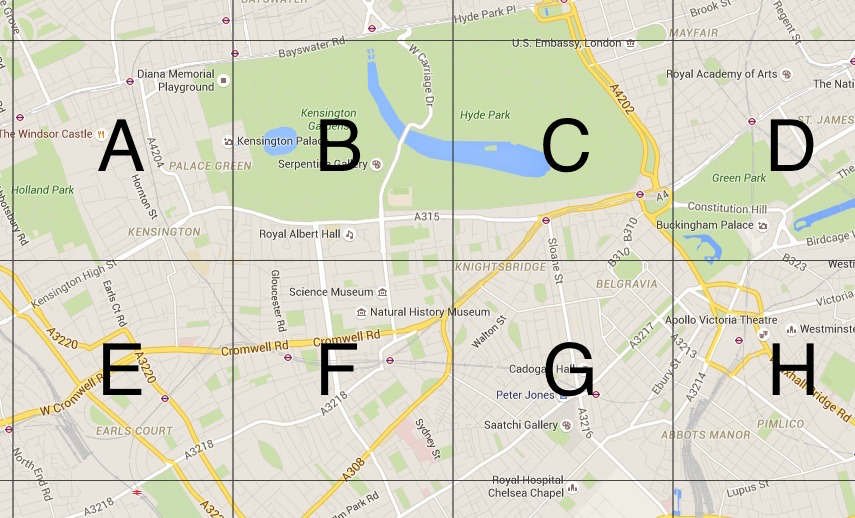
\includegraphics[scale=.4]{C3/mapgrid}
\caption{Example of a predefined square grid map}
\end{figure}

\begin{figure}[ht]
\centering
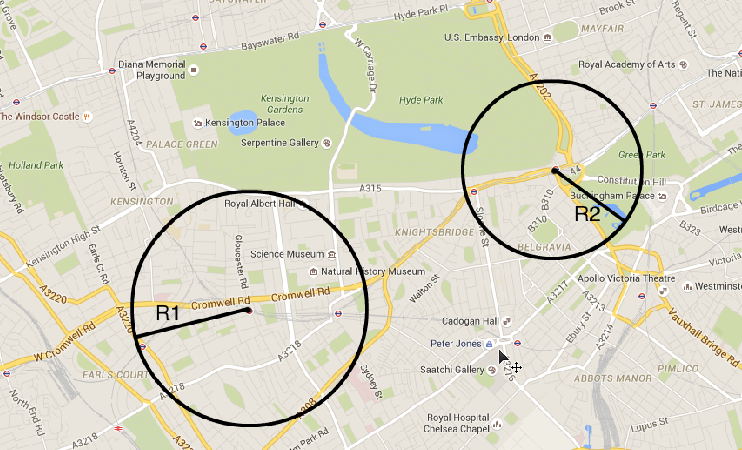
\includegraphics[scale=.46]{C3/mapclusters}
\caption{Example of a cluster map}
\end{figure}

\section{Project Milestones}
The main milestones of the projects will be the following:
\begin{enumerate}
\item \textbf{Centralised user data market}, that will do the following:
	\begin{itemize}
    \item Set up end-to-end skeleton of the proof of concept, with a centralised collection point of the location data, the latter being transmitted in an encrypted manner.
    \item Use \textit{Map 1}, a basic square grid map from which the data is collected. (See \textit{3.1.2. Map Milestones} for further details.)
    \item Run basic functions over the set of collected data, such as a count or sum function, mainly answering the question of 'How many users entered/exited the $X$ grid?', where $X$ will be a predefined square grid in the map.\end{itemize}
\item \textbf{Quasi-decentralised user data market}, where intermediate collectors abstract away any meta-information that can be inferred from the raw set of upload times. This system will trust the intermediate collectors to behave correctly, focusing on the following:
\begin{itemize}
\item Exploring the implied threat model in order to better understand the coupling between the users and the server that runs the data computations.
\item Try out different subscription models on the client side (i.e. a smartphone user sending out encrypted data to the same intermediate data collector vs. varying in a certain way the data collector choice.)
\end{itemize}
\item \textbf{Completely decentralised user data market}, where statistical knowledge can be mined from the collected user data that is stored (encrypted) only on the smartphone where it has been produced.
\end{enumerate}

\section{Project Timeline}
By starting the work on the implementation on February 1st, the project initially proposed timeline is the following:

\begin{center}
  \begin{tabular}{| c | c | c |}
    \hline
    Approx. Deadline & Task & No. of weeks \\ \hline
    29.02 & First version of M1 & 4 \\ 
    07.03 & Testing the M1 system & 1 \\ \hline
    04.04 & First version of M2 & 4 \\
    11.04 & Testing the M2 system & 1 \\
    18.04 & Study variations on M2 & 1 \\ \hline
    09.05 & First version of M3 & 3 \\
    16.05 & Testing the M3 version & 1 \\ \hline
    23.05 & Implement the lottery system & 1 \\ \hline
    06.06 & More refined testing & 2 \\ \hline
    20.06 & System evaluation & 2 \\ 
    24.06 & Finalise the report and presentation & 1 \\
    \hline
  \end{tabular}
\bigskip
\\
Table 3.1: Initially proposed timeline, highlighting the general tasks and milestones \\ to be achieved.
\end{center}
\section{To Be Used Technologies}
Due to the novelty of the quest the project is trying to solve, there will obviously be a lot of research into what technologies can be relevant in achieving the proposed goals. Currently, the focus is on CryptDB \cite{cryptdb}, and secure multi-party computations for privacy preserving data mining \cite{smpc}, that will be expanded in the final report.